%% Detecting Cross-Use-Case Inconsistencies in Industrial Dataspace Ontologies
%% ISWC 2026 Workshop Full Research Paper
%% CEUR-WS single-column format (ceurart class)
%%
%% ── Page Budget (full research paper, body 8-12 pages + refs separate) ──
%%   Section 1  Introduction          ~1.00 page
%%   Section 2  Background            ~0.75 page
%%   Section 3  Related Work          ~1.00 page
%%   Section 4  Methodology           ~1.00 page
%%   Section 5  Findings              ~4.50 pages  (main contribution)
%%   Section 6  Discussion            ~1.50 pages
%%   Section 7  Conclusion            ~0.75 page
%%   Body total                       ~10.50 pages (within 8-12 limit)
%%   References                       excluded from page limit
%%
\documentclass[]{ceurart}

\sloppy

\usepackage{listings}
\lstset{breaklines=true}
\usepackage{booktabs}
\usepackage{graphicx}
\usepackage{xcolor}

%%
%% end of the preamble, start of the body of the document source.
\begin{document}

%%
%% Rights management information.
\copyrightyear{2026}
\copyrightclause{Copyright for this paper by its authors.
  Use permitted under Creative Commons License Attribution 4.0
  International (CC BY 4.0).}

%%
%% Conference information
\conference{SemIIM 2026: 4th International Workshop on Semantic Industrial
  Information Modelling, co-located with ISWC 2026, October 25--29, 2026, Bari, Italy}

%%
%% Title
\title{Detecting Cross-Use-Case Inconsistencies in Industrial Dataspace Ontologies:
  An Empirical Study of 123 Catena-X Aspect Models}

%%
%% Authors
\author[1]{Sangil Lee}[%
  orcid=0009-0001-8320-9728,
  email=sgslee7@liverpool.ac.uk,
]
\cormark[1]
%% TODO: Add co-authors if applicable
% \author[2]{Co-Author Name}[%
%   orcid=0000-0000-0000-0000,
%   email=coauthor@example.com,
% ]

\address[1]{Department of Computer Science, University of Liverpool, Liverpool, UK}
% \address[2]{Affiliation 2, City, Country}

\cortext[1]{Corresponding author.}

%%
%% Abstract
\begin{abstract}
  Catena-X, a European data space initiative for the automotive industry, defines 123
  Aspect Models using the Semantic Aspect Meta Model (SAMM) to standardize data
  exchange across use cases such as Traceability, Product Carbon Footprint (PCF),
  Digital Product Passport (DPP), and Quality Management. However, as these
  models were developed independently by different working groups, semantically
  equivalent data properties---such as part identification, manufacturing
  information, and material composition---are often defined with incompatible
  types, structures, or naming conventions across use case boundaries. This
  fragmentation creates concrete interoperability barriers for organizations
  that must implement multiple use cases simultaneously.

  We present a systematic methodology for automatically detecting
  and classifying cross-use-case property overlaps across the entire Catena-X
  Aspect Model corpus. Analyzing 123 models (2{,}217 properties), we identify
  249 overlapping property names, of which 40 exhibit type-level conflicts. We
  introduce a three-tier classification---IDENTICAL, COMPATIBLE, and
  CONFLICT---and provide in-depth case studies of critical conflicts, including
  the Battery Pass vs.\ Digital Product Passport model pair where EU regulatory
  divergence (Battery Regulation 2023/1542 vs.\ ESPR 2024/1781) manifests as
  incompatible ontological structures. Our findings provide the first
  quantified evidence of a theoretically expected pattern: regulatory
  divergence creating structural fault lines in modular industrial
  ontologies. We discuss implications for Catena-X governance and for the
  broader landscape of multi-jurisdictional data ecosystems.
\end{abstract}

%%
%% Keywords
\begin{keywords}
  Catena-X \sep
  SAMM \sep
  Aspect Models \sep
  Ontology Modularization \sep
  Semantic Interoperability \sep
  Digital Product Passport \sep
  Regulatory Ontology \sep
  Automotive Data Ecosystems
\end{keywords}

\maketitle

%% ===================================================================
%% SECTION 1: Introduction  (~1.00 page)
%% ===================================================================
\section{Introduction}\label{sec:introduction}

%% ── Step 1: Hook — regulatory motivation ──
The European automotive industry is undergoing a transformation toward
shared data ecosystems, driven by regulatory frameworks such as the EU
Battery Regulation 2023/1542~\cite{eu2023battery} and the Ecodesign for
Sustainable Products Regulation (ESPR) 2024/1781~\cite{eu2024espr}.
These regulations mandate digital traceability and product passports
across the supply chain, creating an unprecedented need for semantic
interoperability among thousands of organizations exchanging
standardized data about parts, materials, and manufacturing processes.

%% ── Step 2: Catena-X introduction ──
Catena-X, the European automotive data space
initiative~\cite{catenax2024models}, addresses this need through a
federated architecture grounded in 123 standardized \emph{Aspect Models}
defined using the Semantic Aspect Meta Model
(SAMM)~\cite{samm2024, cx0003samm}. Each Aspect Model represents a
logical view of data exchanged for a specific use
case---Traceability, Digital Product Passport (DPP), Quality Management,
Product Carbon Footprint (PCF)---developed independently by domain
working groups within the Catena-X ecosystem.

%% ── Step 3: Problem statement ──
This independent development creates a hidden interoperability
challenge: semantically equivalent concepts---part identification,
manufacturing information, material composition---are often modeled
with incompatible types or structures across use case boundaries. The
challenge intensifies when different use cases must satisfy different
external regulatory requirements: a property named \texttt{materials}
answers the question ``What hazardous substances are present?'' under
the Battery Regulation, but answers ``What is the recycled content?''
under ESPR. While the Catena-X standard
CX-0143~\cite{cx0143dpp} explicitly recommends reuse of generic DPP
modules, no automated mechanism currently verifies cross-model
consistency, and the community has identified this as an open governance
challenge~\cite{catenax2024issue720}.

%% ── Step 4: Research question ──
This raises the empirical question: \emph{How prevalent are
property-level inconsistencies across the Catena-X Aspect Model corpus,
and to what extent does regulatory divergence drive these
inconsistencies?}

%% ── Step 5: Approach + Contributions ──
We address this question through a systematic empirical analysis of all
123 Catena-X Aspect Models (2{,}217 properties in 279 Turtle files),
classifying cross-use-case overlaps into three structural
tiers---IDENTICAL, COMPATIBLE, and CONFLICT---and conducting in-depth
case studies of the most critical conflicts.

This paper makes three contributions:
\begin{enumerate}
  \item The first systematic empirical analysis of cross-use-case
    property overlap across 123 Catena-X Aspect Models, comprising
    2{,}217 properties and 249 cross-model overlaps. To our knowledge,
    this is the first quantitative measurement of inter-model consistency
    in an industrial dataspace ontology at this scale.
  \item A three-tier overlap taxonomy (IDENTICAL, COMPATIBLE,
    CONFLICT) with an automated detection pipeline, grounded
    in established modular ontology
    theory~\cite{oh2009ontology, stuckenschmidt2009modular} but
    specialized for SAMM's two-level type structure (Characteristic +
    dataType).
  \item In-depth case studies---including the Battery Pass and Digital
    Product Passport pair---revealing that regulatory-driven structural
    divergence accounts for at least half of the true conflicts in our
    validated sample. Grounded in modular ontology theory and our
    empirical findings, we argue that regulatory-driven structural
    divergence constitutes a systematic challenge for modular ontologies operating
    under heterogeneous regulatory regimes, with implications beyond
    Catena-X.
\end{enumerate}

%% ===================================================================
%% SECTION 2: Background  (~0.75 page)
%% ===================================================================
\section{Background}\label{sec:background}

SAMM~\cite{samm2024} is a meta-model built on RDF/Turtle that defines the
structural primitives for Catena-X Aspect Models. Its core concepts are:
\textbf{Aspect} (the top-level model), \textbf{Property} (a named data
attribute), \textbf{Characteristic} (the type contract of a Property, e.g.,
\texttt{Text}, \texttt{Timestamp}, or a custom type), \textbf{Entity} (a
structured complex type referenced by a Characteristic), and \textbf{Trait}
(a Characteristic with added constraints such as regex patterns or value
ranges)~\cite{cx0003samm}.

A key design feature of SAMM is its \emph{two-level type system}: a
Property's effective data type is determined by its Characteristic, which
either maps to an \texttt{xsd} primitive (e.g., \texttt{xsd:string},
\texttt{xsd:dateTime}) or references a complex Entity definition with its
own nested Properties. This two-level indirection---Property $\to$
Characteristic $\to$ dataType---means that two properties sharing the same
name may agree on the Characteristic class but diverge on the underlying
dataType, or vice versa. This distinction is central to our three-tier
overlap classification (Section~\ref{sec:findings-taxonomy}).

SAMM models may reference definitions from other models via namespace
imports, enabling reuse of shared Characteristics and Entities across use
cases. However, imports are version-pinned: a model importing
\texttt{v5.0.0} of another model's namespace will not automatically receive
changes introduced in \texttt{v6.0.0} or later, creating potential
compatibility drift when the imported model evolves independently.

The Catena-X model corpus~\cite{catenax2024models} is maintained in a public
GitHub repository organized as a flat namespace: each model resides in a
directory named \texttt{io.catenax.\{domain\}.\allowbreak\{model\_name\}},
with versioned subdirectories containing Turtle files and a
\texttt{metadata.json} file indicating status (\texttt{release},
\texttt{draft}, or \texttt{deprecated}). As of our analysis, the repository
contains 123 models (109~release, 14~draft/other) spanning use case domains
including Traceability, PCF, DPP, Quality Management, Supply Chain
Management, and Circular Economy. Twenty shared modules
(\texttt{io.catenax.shared.*}) provide reusable definitions, though their
adoption varies across use cases. Each domain is governed by an independent
working group, and no automated mechanism enforces cross-domain property
consistency.

%% ===================================================================
%% SECTION 3: Related Work  (~1.00 page)
%% ===================================================================
\section{Related Work}\label{sec:related-work}

\paragraph{Modular ontology design.}
The challenge of maintaining consistency across modular ontologies is
well-established. Shimizu et al.~\cite{shimizu2023modular} formalize
Modular Ontology Modeling (MOM) with patterns for module composition,
while Stuckenschmidt et al.~\cite{stuckenschmidt2009modular} address
knowledge modularization theory. Oh and Ahn~\cite{oh2009ontology}
propose cohesion and coupling metrics for ontology modules, and
Keet~\cite{keet2023modular} provides a comprehensive treatment of
ontology engineering principles including modularization. These works
establish theoretical foundations but do not empirically analyze
large-scale industrial ontology corpora for cross-module consistency.

\paragraph{Industrial semantic modeling.}
Recent workshop contributions have addressed semantic modeling for
industrial data exchange, both through integration
architectures~\cite{grangel2023datamesh, milicicbrandt2023imf} and
domain-specific vocabularies~\cite{tsalapati2023shm, yahya2023camcont,
kebede2024semantic}. However, each operates within a single domain and
does not examine cross-domain consistency within a shared
ecosystem---the central focus of our work.

\paragraph{DPP ontologies and Catena-X.}
The Digital Product Passport has motivated ontology network design.
Jansen et al.~\cite{jansen2024designing} design an ontology network for
DPPs using modular ontology patterns, proposing a top-level structure
that connects product, process, and regulatory concepts. Deich et
al.~\cite{deich2025dpp} address the complementary problem of connecting
general DPP frameworks with domain-specific information sources,
demonstrating mappings between DPP ontologies and building information
models. Both works focus on \emph{designing} coherent ontology structures
but do not empirically measure whether existing deployed models actually
achieve consistency. St\"{a}bler et al.~\cite{staebler2023amcis} come
closest to our concern by identifying ``ontological dissonance'' in
ecosystem platforms using network graph analysis, though their approach
operates at the model level rather than the property level and does not
quantify type-level conflicts. Ishihara and
Matsutsuka~\cite{ishihara2025interoperable} compare data space
implementations between Japan and Europe, confirming that cross-border
interoperability challenges mirror the cross-use-case challenges we
examine within a single ecosystem.

\paragraph{Gap.}
Existing work addresses either inter-ontology alignment (across different
ontologies) or domain-specific modeling (within a single use case).
What remains unexamined is \emph{intra-ecosystem cross-use-case
consistency}---whether independently developed models within the same
data space define overlapping concepts consistently. Our work fills this
gap with the first corpus-wide empirical analysis of property-level
overlaps across Catena-X Aspect Models.

%% ===================================================================
%% SECTION 4: Methodology  (~1.00 page)
%% ===================================================================
\section{Methodology}\label{sec:methodology}

\subsection{Data Collection}\label{sec:data-collection}

We cloned the Catena-X Semantic Models
repository~\cite{catenax2024models} and selected the latest release
version of each model. When no release version existed, we used the
latest available version regardless of status. This yielded 123 models
(109~release, 14~draft/other) containing 279 Turtle files.

\subsection{Property Extraction}\label{sec:extraction}

We built a Python pipeline using RDFLib~\cite{rdflib2024} that parses
each model's Turtle files and extracts all SAMM Property instances. The
pipeline handles both SAMM 2.0.0 and 2.1.0 namespace URIs, which coexist
in the corpus. For each property, we extract: \texttt{local\_name} (the
fragment identifier), \texttt{preferredName}, \texttt{description},
\texttt{characteristic} (the Characteristic class name),
\texttt{dataType} (the resolved \texttt{xsd} type or Entity name), and
\texttt{exampleValue}. Properties imported from external namespaces
(e.g., \texttt{io.catenax.shared.*}) are excluded from the defining
model's count to avoid double-counting shared definitions.

\subsection{Overlap Detection and Classification}\label{sec:classification}

We group all extracted properties by \texttt{local\_name} across models.
Properties appearing in two or more models constitute an overlap.
Each overlap is classified into one of three tiers:

\begin{itemize}
  \item \textbf{IDENTICAL}: same Characteristic class \emph{and} same
    \texttt{xsd} dataType across all models.
  \item \textbf{COMPATIBLE}: same dataType but differently named
    Characteristics.
  \item \textbf{CONFLICT}: different dataTypes or structurally
    incompatible Entity definitions.
\end{itemize}

\subsection{Manual Validation}\label{sec:validation}

To assess the semantic significance of detected conflicts, we manually
examined the top~10 CONFLICT properties (ranked by affected model count).
For each, we compared \texttt{preferredName}, \texttt{description}, and
Entity structure across models to distinguish \emph{true conflicts}
(same real-world concept, incompatible types) from \emph{coincidental
name collisions} (unrelated concepts sharing a generic name) and
\emph{domain-justified divergences} (intentionally different types
satisfying distinct external standards).

%% ===================================================================
%% SECTION 5: Findings  (~4.50 pages — main contribution)
%% ===================================================================
\section{Findings}\label{sec:findings}

%% ── 5.1 Quantitative Overview (~0.5 page) ──────────────────
\subsection{Quantitative Overview}\label{sec:findings-quant}

We applied the extraction pipeline described in Section~\ref{sec:methodology}
to the 123 Catena-X Aspect Models (latest release version per model),
parsing 279 Turtle files containing a total of 2{,}217 SAMM Property
definitions. Table~\ref{tab:summary} summarizes the corpus-level statistics.

\begin{table}[h]
  \caption{Corpus-level statistics of the Catena-X Aspect Model analysis.}
  \label{tab:summary}
  \begin{tabular}{lr}
    \toprule
    Metric & Value \\
    \midrule
    Aspect Models analyzed           & 123 \\
    \quad of which \textit{release}  & 109 \\
    \quad of which \textit{draft/other} & 14 \\
    Shared modules (\texttt{io.catenax.shared.*}) & 20 \\
    Turtle files parsed              & 279 \\
    Properties extracted             & 2{,}217 \\
    Unique property names            & 1{,}759 \\
    Overlapping property names ($\geq$2 models) & 249 (14.2\%) \\
    \quad IDENTICAL                  & 114 \\
    \quad COMPATIBLE                 & 95 \\
    \quad CONFLICT                   & 40 \\
    \bottomrule
  \end{tabular}
\end{table}

Of the 1{,}759 unique property names, 249 (14.2\%) appear in two or more
models. While the majority of these overlaps are structurally
consistent---114 IDENTICAL (same Characteristic and dataType) and 95
COMPATIBLE (same dataType, different Characteristic name)---40 property
names exhibit type-level conflicts where the same name maps to different
\texttt{xsd} dataTypes or structurally incompatible Entity definitions
across models.

Table~\ref{tab:top-conflicts} lists the most severe conflicts ranked by
the number of affected models. The property \texttt{value} appears in 13
models with four distinct dataTypes (\texttt{string}, \texttt{double},
\texttt{float}, \texttt{integer}), while \texttt{partTypeInformation}
spans 7 models with two incompatible Entity structures.

\begin{table}[h]
  \caption{Top CONFLICT properties by number of affected models.
    Entity-typed properties are counted by Entity name; properties
    using SAMM built-in Characteristics without an explicit
    \texttt{xsd} dataType are excluded from the count.}
  \label{tab:top-conflicts}
  \begin{tabular}{lrrp{4.5cm}}
    \toprule
    Property & Models & DataTypes & Example types \\
    \midrule
    \texttt{value}       & 13 & 4 & string, double, float, integer \\
    \texttt{quantity}    &  8 & 2 & Quantity (entity), float \\
    \texttt{partTypeInformation} & 7 & 2 & PartTypeInformationEntity, PartTypeEntity \\
    \texttt{key}         &  7 & 2 & anyURI, string \\
    \texttt{version}     &  6 & 3 & VersionEntity, string, nonNegativeInteger \\
    \texttt{weight}      &  5 & 2 & \{value,unit\} entity vs.\ scalar double/float \\
    \texttt{childItems}  &  5 & 2 & ChildData, ChildItemEntity \\
    \texttt{type}        &  5 & 3 & CertificateTypeEntity, TypeEntity, string \\
    \texttt{changedAt}   &  5 & 2 & dateTime, dateTimeStamp \\
    \bottomrule
  \end{tabular}
\end{table}

\paragraph{Overlap distribution.}
The distribution of overlapping properties exhibits a strong long tail:
155 of 249 overlapping properties (62.2\%) are shared by exactly 2~models,
while only 25 (10.0\%) appear in 5 or more models
(Figure~\ref{fig:overlap-dist}). The mean model count per overlapping
property is 2.84 (median~2, $\sigma$~=~1.72). Notably, the proportion of
CONFLICT classifications increases with model count: among properties
shared by 2~models, 11.0\% are CONFLICT (17/155), while among properties
shared by 5+~models, 24.0\% are CONFLICT (6/25). This suggests that
widely reused property names face greater type divergence pressure as
more working groups independently define them.

\begin{figure}[h]
  \centering
  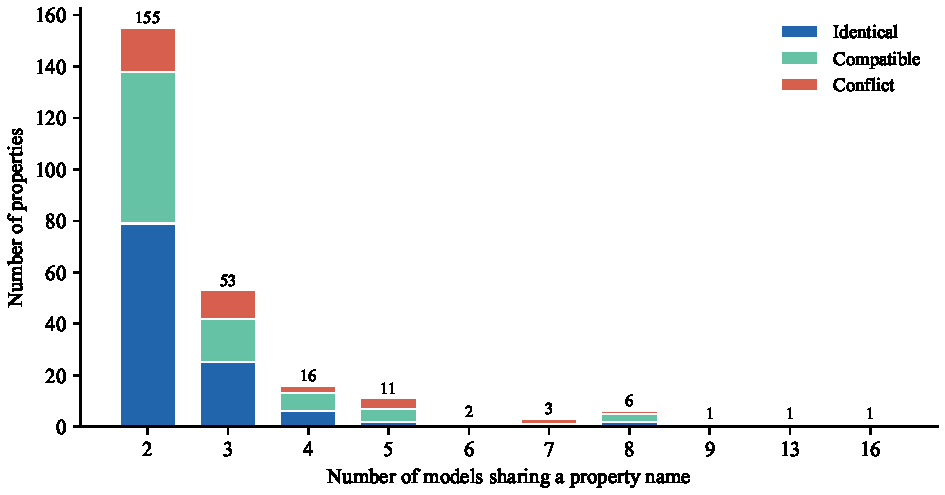
\includegraphics[width=0.85\columnwidth]{figures/overlap_distribution.pdf}
  \caption{Distribution of overlapping properties by number of models
    sharing the same property name, broken down by overlap classification.}
  \label{fig:overlap-dist}
\end{figure}

\paragraph{Conflict type breakdown.}
Of the 40 CONFLICT properties, 15 (37.5\%) involve incompatible Entity
definitions, 12 (30.0\%) involve \texttt{xsd} dataType disagreements,
and 13 (32.5\%) are \emph{mixed} conflicts where some models use a
primitive type while others use a complex Entity---the most severe form
of structural incompatibility (e.g., \texttt{quantity} is a scalar
\texttt{float} in some models but a structured \texttt{Quantity} entity
with \texttt{value} and \texttt{unit} fields in others).

\paragraph{Cross-domain conflict analysis.}
To understand whether conflicts arise from independent modeling by
different teams or from divergence within a single domain, we mapped each
model to one of nine use-case domains (Traceability, DPP, PCF, Quality,
Supply Chain, Circular Economy, Manufacturing, Shared, and Other) and
classified each conflict as cross-domain or within-domain. Of the 40
CONFLICT properties, 32 (80.0\%) involve models from \emph{different}
domains, while only 8 (20.0\%) are within-domain conflicts---5 of which
occur within the DPP domain (between Battery Pass, Electric Drive
Passport, and Transmission Pass sub-models). The domain pairs with the
most conflicts are Circular Economy--Other (9), Circular Economy--Shared
(7), and DPP--Other (5), suggesting that domains with the least
alignment to shared vocabularies are most prone to property conflicts.

%% ── 5.2 Severity Taxonomy (~0.5 page) ─────────────────────
\subsection{Overlap Classification and Severity}\label{sec:findings-taxonomy}

Our three-tier classification captures structurally distinct overlap
patterns. We define each tier and illustrate with examples from the corpus:

\paragraph{IDENTICAL.} The same property local name maps to the same
Characteristic class and the same \texttt{xsd} dataType across all models
in which it appears. For example, \texttt{description} uses the
\texttt{Text} Characteristic with \texttt{xsd:string} in all 8~models
that define it. These overlaps represent successful de facto
standardization, even when models do not explicitly import a shared
definition.

\paragraph{COMPATIBLE.} The property shares the same dataType across models
but uses differently named Characteristics. For instance,
\texttt{catenaXId} appears in 16~models, always representing a Catena-X
UUID identifier, but through Characteristics named \texttt{UuidV4Trait}
(13~models) or \texttt{CatenaXIdTrait} (3~models). Notably, even this
identifier---required by the Industry Core KIT~\cite{cxindustrycore} and arguably the most
fundamental shared concept in the ecosystem---exhibits Characteristic
divergence. While data-level interoperability is preserved, schema-level
tooling cannot automatically recognize these as equivalent without
additional mapping.

\paragraph{CONFLICT.} The property name maps to different dataTypes or
structurally incompatible Entity definitions across models. We further
distinguish two sub-categories through manual validation:

\begin{itemize}
  \item \textbf{True conflict:} Properties that represent the same
    real-world concept but are modeled with incompatible types. Example:
    \texttt{weight} represents physical mass in all five models, but three
    use a complex \texttt{\{value, unit\}} entity via
    \texttt{MassCharacteristic}, while two use a scalar
    \texttt{xsd:double}/\texttt{float} with a fixed kilogram unit.
    A second critical true conflict is \texttt{partTypeInformation},
    which appears in 7~models with two incompatible Entity definitions:
    \texttt{PartTypeInformationEntity} (used by 6
    Traceability/Planning models) includes
    \texttt{partClassification}, while DPP's \texttt{PartTypeEntity}
    omits it to align with ESPR 2024/1781~\cite{eu2024espr}, creating a structurally
    incompatible simplification.
  \item \textbf{Domain-justified divergence:} Properties where the name
    collision is coincidental or where different types are intentionally
    chosen to satisfy distinct domain standards. Example: \texttt{version}
    uses \texttt{xsd:nonNegativeInteger} in the PCF model (mandated by
    WBCSD/PACT~\cite{wbcsd2024pact}), \texttt{xsd:string} with SemVer constraint in the message
    header, and a complex \texttt{VersionEntity} in engineering master data.
    These represent three genuinely different concepts that happen to share a
    name.
\end{itemize}

\noindent
Distinguishing true conflicts from domain-justified divergences is
essential because the corrective action differs: true conflicts demand
harmonization or shared module reuse, while domain-justified divergences
indicate that property names should be qualified with domain-specific
prefixes (e.g., \texttt{footprintVersion}, \texttt{messageVersion}) rather
than left ambiguous.

Of the 40 CONFLICT properties, our manual examination of the top 10 (by
model count) identified approximately 6 as true conflicts and 4 as
domain-justified divergences (where same-named properties intentionally
use different types to satisfy distinct domain standards).

\paragraph{Theoretical grounding.}
Our classification draws on Oh and Ahn's~\cite{oh2009ontology}
cohesion-coupling tension in modular ontologies, specializing it for
SAMM's two-level type system: where they measure cohesion within a
single module, we measure \emph{consistency across modules} sharing a
property name. The IDENTICAL/COMPATIBLE/CONFLICT distinction parallels
Stuckenschmidt et al.'s~\cite{stuckenschmidt2009modular} structural
vs.\ semantic compatibility, applied at the property level.

%% ── 5.3 Case Study: Battery Pass <-> DPP (~1.0 page) ──────
\subsection{Case Study: Battery Pass and Digital Product Passport}%
\label{sec:findings-case-study}

We selected the Battery Pass (BP, v6.1.0) and Digital Product Passport
(DPP, v7.0.0) model pair for in-depth analysis because (1)~they share 9
property names, making them the highest-overlap cross-domain pair in the
corpus; (2)~both implement EU regulatory requirements, making their
relationship a concrete test of standard compliance; and (3)~the Catena-X
standard CX-0143~\cite{cx0143dpp} explicitly positions BP as a
domain-specific extension of the generic DPP framework. This pair represents a critical instance where structural divergence
coincides with regulatory divergence. Of the approximately 6 true
conflicts identified among the top~10 most-affected CONFLICT properties
(Section~\ref{sec:findings-taxonomy}), at least 3 coincide with
differences in EU regulatory requirements (Battery Regulation
2023/1542~\cite{eu2023battery}, ESPR
2024/1781~\cite{eu2024espr}). These span two distinct case patterns:
\texttt{materials} and \texttt{characteristics} in the BP--DPP pair,
plus \texttt{partTypeInformation} across Traceability, Planning, and
DPP models. Together, they account for at least half of the true
conflicts in this validated subset.

\paragraph{Import relationship.}
Battery Pass v6.1.0 imports the DPP namespace at version 5.0.0, but
the current DPP release is v7.0.0---two major versions ahead. Properties
added or modified in DPP v6.0.0 and v7.0.0 are invisible to Battery Pass
consumers, creating a silent compatibility drift.

\paragraph{Shared property classification.}
Table~\ref{tab:bp-dpp} classifies the 9 shared properties. Seven are
IDENTICAL (both models use the same Characteristic and Entity name) and
two exhibit CONFLICT: \texttt{characteristics} and \texttt{materials}.

\begin{table}[h]
  \caption{Shared properties between Battery Pass (v6.1.0) and Digital
    Product Passport (v7.0.0).}
  \label{tab:bp-dpp}
  \begin{tabular}{lllc}
    \toprule
    Property & BP type & DPP type & Class \\
    \midrule
    operation       & OperationEntity       & OperationEntity       & IDENT \\
    sustainability  & SustainabilityEntity  & SustainabilityEntity  & IDENT \\
    physicalDimension & PhysDimensionEntity & PhysDimensionEntity   & IDENT \\
    specVersion     & Text                  & Text                  & IDENT \\
    sources         & SourceList            & SourceList            & IDENT \\
    carbonFootprint & FootprintList         & FootprintList         & IDENT \\
    identification  & IdentificationEntity  & IdentificationEntity  & IDENT \\
    \textbf{characteristics} & \textbf{CharacteristicsEntity} & \textbf{ProductCharEntity} & \textbf{CONFL} \\
    \textbf{materials}       & \textbf{ChemicalMaterialEntity} & \textbf{MaterialEntity} & \textbf{CONFL} \\
    \bottomrule
  \end{tabular}
\end{table}

\paragraph{Conflict analysis: \texttt{characteristics}.}
Battery Pass defines \texttt{characteristics} as an entity with two
properties: \texttt{warranty} and \texttt{physicalDimension}. DPP defines
it with five properties: \texttt{lifespan}, \texttt{physicalDimension},
\texttt{physicalState}, \texttt{generalPerformanceClass}, and
\texttt{otherCharacteristics}. While \texttt{physicalDimension} appears in
both, the surrounding structure is incompatible---a system consuming DPP
data cannot parse BP's \texttt{characteristics} without transformation, and
vice versa.

\paragraph{Conflict analysis: \texttt{materials}.}
The divergence in \texttt{materials} reveals a deeper semantic conflict
rooted in regulatory differences. Battery Pass, governed by the Battery
Regulation (EU) 2023/1542~\cite{eu2023battery}, models materials as
chemical composition: \texttt{activeMaterials}, \texttt{hazardousSubstance},
and \texttt{materialComposition} (3~properties). DPP, governed by the
Ecodesign for Sustainable Products Regulation (ESPR) (EU)
2024/1781~\cite{eu2024espr}, models materials from a circular economy
perspective: \texttt{recycled}, \texttt{materialType},
\texttt{materialOrigin}, \texttt{substancesOfConcernInformation}, and
7~additional properties (10+~total). The same property name
\texttt{materials} answers fundamentally different regulatory questions:
``What hazardous substances does this battery contain?'' vs.\ ``What is the
recycled content percentage of this product?''

\paragraph{Regulatory roots of ontological divergence.}
The structural conflicts between BP and DPP align with fundamental
differences in their governing regulations. The Battery Regulation (EU)
2023/1542 targets a specific product category (batteries and waste
batteries) and mandates detailed chemical composition disclosure,
including critical raw materials and hazardous substances. The ESPR (EU)
2024/1781, by contrast, is a horizontal framework regulation applicable
to all products placed on the EU market, emphasizing circular economy
metrics such as recycled content, durability, and repairability. Although
both regulations require digital product passports and share a 2027
implementation timeline, they address different policy objectives---chemical
safety and raw material traceability for batteries vs.\ circular economy
metrics for all products---creating divergent data requirements.
Within Catena-X, these regulations are implemented by separate working
groups (Battery Passport WG and DPP WG) with independent development
cycles, as evidenced by the version gap between BP's import of DPP
v5.0.0 and the current DPP v7.0.0 release. This organizational
separation correlates with the regulatory separation, though we note
that establishing a causal link would require comparative analysis
across multiple regulatory pairs and ecosystems.

\paragraph{Broader implications.}
The BP--DPP case instantiates a general theoretical concern: when modules
answer to different external normative sources, the module boundary becomes
a structural fault line rather than a clean interface. Empirical
verification in other ecosystems remains future work.

%% ── 5.4 Limitations ───────────────────────────────────────
\subsection{Limitations}\label{sec:findings-limits}

We identify three methodological limitations, each suggesting a
direction for future work.

\paragraph{L1: Name-based detection.}
Our pipeline relies on property local name matching, which introduces
both false positives and false negatives. Generic property names such as
\texttt{value} (13~models) and \texttt{key} (7~models) represent
coincidental name collisions---distinct concepts that happen to share a
name across unrelated domains. For example, \texttt{value} denotes a
monetary amount in \texttt{customs\_information}, a measurement result in
\texttt{certificate\_of\_analysis}, and a key-value pair value in
\texttt{serial\_part}. Of the 40 CONFLICT properties, we estimate that
approximately 10--15 fall into this category, distinct from the
domain-justified divergences identified in
Section~\ref{sec:findings-taxonomy} where the name collision is
intentional. Conversely, semantically equivalent properties with different
names are invisible to our pipeline. For example,
\texttt{manufacturerPartId} (defined locally in 4~models) and
\texttt{partId} could represent the same concept but would not be
detected as overlapping.

\paragraph{L2: Cross-version analysis.}
Our pipeline analyzes only the latest release version of each model.
However, cross-model imports may reference older versions, as
demonstrated by the Battery Pass importing DPP v5.0.0 while v7.0.0 is
current (Section~\ref{sec:findings-case-study}). A comprehensive analysis
should compare all version pairs referenced by cross-model imports to
identify version-induced compatibility gaps.

\paragraph{L3: Semantic similarity.}
Our detection is purely syntactic (property local name matching).
NLP-based semantic similarity analysis on \texttt{preferredName} and
\texttt{description} fields could detect additional overlaps among
differently named but semantically equivalent properties (e.g.,
\texttt{productionDate} and \texttt{date} labeled ``Production Date'' in
\texttt{serial\_part}). Quantifying these false negatives would provide a
more complete picture of the true overlap landscape.

\paragraph{Implications.}
These limitations suggest that the 40 CONFLICT figure represents a lower
bound for true interoperability issues (undetected semantic overlaps)
while simultaneously overstating severity (coincidental name collisions).
A more precise estimate would require NLP-based description similarity
and multi-rater validation.

%% ===================================================================
%% SECTION 6: Discussion  (~1.50 pages)
%% ===================================================================
\section{Discussion}\label{sec:discussion}

\subsection{Governance Implications for Catena-X}

Our findings suggest four concrete recommendations for the Catena-X
model governance process:

\begin{enumerate}
  \item \textbf{Domain-prefixed naming} for generic property names.
    Properties like \texttt{version} and \texttt{value} should carry
    domain prefixes (e.g., \texttt{footprintVersion},
    \texttt{passportVersion}) to avoid coincidental name collisions.
  \item \textbf{Mandatory shared Characteristic reuse} for common
    concepts. The 20 existing shared modules
    (\texttt{io.catenax.shared.*}) are underutilized---for example,
    \texttt{weight} is defined with three incompatible patterns across
    five models despite a shared physical dimension module being
    available.
  \item \textbf{Cross-model consistency checks} integrated into the
    CI/CD pipeline. Our detection pipeline could be adapted as a GitHub
    Actions check that flags new CONFLICT properties before merge.
  \item \textbf{Version dependency tracking} for cross-model imports.
    The Battery Pass importing DPP v5.0.0 while v7.0.0 is current
    (Section~\ref{sec:findings-case-study}) illustrates the need for
    automated dependency staleness alerts.
\end{enumerate}

\subsection{Impact on Multi-Use-Case Implementers}

The 40 type-level conflicts have practical consequences for organizations
implementing multiple Catena-X use cases. Each conflict requires manual
data mapping or transformation logic, and the effort multiplies with the
number of use cases adopted. For example, an organization implementing
Traceability, DPP, and PCF simultaneously must build a scalar-to-entity
adapter for \texttt{quantity} between PCF (scalar \texttt{float}) and
Traceability (structured \texttt{Quantity} entity with \texttt{value}
and \texttt{unit} fields). These mapping layers accumulate silently and
become a maintenance burden when upstream models release new versions.

This burden falls disproportionately on SMEs---Tier~2/3 automotive
suppliers who lack dedicated semantic engineering teams and rely on
off-the-shelf connectors that assume structural consistency across
models. The 80\% cross-domain conflict rate
(Section~\ref{sec:findings-quant}) suggests that this assumption is
systematically violated.

\subsection{Generalizability}

We distinguish two dimensions of generalizability: methodological and
empirical.

\paragraph{Methodology.}
Our pipeline is applicable to any modular ontology ecosystem with typed
property definitions on an RDF-based meta-model; adapting it requires
only replacing SAMM-specific namespace resolution. Emerging data space
initiatives such as Manufacturing-X and
Ouranos~\cite{ishihara2025interoperable} adopt similar architectures
and are likely candidates for analogous analysis.

\paragraph{Empirical findings.}
While our empirical evidence is drawn from a single ecosystem, the
underlying mechanism we identify---regulatory divergence creating
structural fault lines at module boundaries---is theoretically
applicable to any modular ontology operating under heterogeneous
regulation. Healthcare data spaces such as the European Health Data
Space (EHDS), which must reconcile cross-border privacy frameworks and
national clinical coding standards, or financial data spaces navigating
tensions between Basel~III and national reporting standards, face
structurally analogous conditions. The Catena-X case provides empirical evidence that this
mechanism manifests concretely at the property level, even when a shared
governance body (Catena-X e.V.) coordinates model development.
Verification in other ecosystems such as Manufacturing-X and Ouranos is
a natural next step.

%% ===================================================================
%% SECTION 7: Conclusion  (~0.75 page)
%% ===================================================================
\section{Conclusion and Future Work}\label{sec:conclusion}

We presented the first systematic empirical analysis of cross-use-case
property overlap across 123 Catena-X Aspect Models. Analyzing 2{,}217
properties, we identified 249 overlapping property names, of which 40
exhibit type-level conflicts. Our three-tier taxonomy---IDENTICAL,
COMPATIBLE, and CONFLICT---provides a principled framework for
classifying overlap severity, and our automated pipeline enables
reproducible detection across evolving model corpora. Through in-depth
case studies of the Battery Pass and Digital Product Passport model pair,
we presented quantified evidence that regulatory-driven structural
divergence---where EU regulations manifest as incompatible ontological
structures---accounts for a substantial portion of the most severe
conflicts in this corpus. We argue that the underlying
mechanism---regulatory divergence creating structural fault lines at
module boundaries---constitutes a systematic challenge for any modular
ontology operating under heterogeneous regulation, warranting
verification across other data space ecosystems.

Future work includes: (1)~longitudinal tracking of property overlap
evolution across model versions; (2)~NLP-based semantic similarity
analysis to detect false negatives (semantically equivalent properties
with different names); (3)~extension of the pipeline to other
SAMM-based ecosystems such as Manufacturing-X; (4)~cross-version
import dependency analysis to identify compatibility gaps between
referenced and current model versions; and (5)~integration
of automated consistency checks into the Catena-X CI/CD governance
pipeline.

%%
%% Acknowledgments
\begin{acknowledgments}
  % TODO: Add funding acknowledgments, advisor thanks, etc.
  % e.g., "This work was supported by ..."
\end{acknowledgments}

%%
%% Bibliography
\bibliography{references}

\end{document}
